\documentclass[preprint,12pt]{article}

\usepackage{algorithmic}
\usepackage{algorithm}
\usepackage{enumerate}
\usepackage{enumitem}
\usepackage{graphics}
\usepackage{graphicx}
\usepackage{geometry}
\usepackage{amsmath}
\usepackage{wrapfig}
\usepackage{subfig}
\usepackage{framed}
\usepackage{color}
\usepackage{bm}

\usepackage{multirow}
\usepackage[T1]{fontenc}
\usepackage[latin9]{inputenc}
%\usepackage{units}
\usepackage{esint}

\geometry{legalpaper,  margin=1in}
%\makeatother

%\usepackage{babel}

\begin{document}
\title{An Empirical Bayesian Framework for Assessing Partisan Bias in Redistricting Plans}

\author{Kevin Baas and Colin McAuliffe}

\maketitle

\begin{abstract}
We present a framework for assessing partisan bias in redistricting plans using an empirical Bayesian approach, as well as a new metric for measuring partisan bias called the specific asymmetry.
Given at least one observation of the election results in a state, we estimate a probability model representing likely future election outcomes.
The expected value of the specific asymmetry is then computed by sampling from the model using the Monte Carlo method.
Redistricting plans which have an expected asymmetry of zero may be considered fair, since on average neither of the two major parties will be given an advantage.
Conversely, redistricting plans which have a nonzero expected asymmetry may be considered to be unfair, since partisan bias is a persistent feature of the plan.
This analysis technique is applied to the United States congressional elections from 1972-2016 to examine the total and net effects of partisan bias in recent history.
We also examine the post 2010 census Wisconsin State Assembly, which is the subject of \emph{Whitford v. Gil}.

\end{abstract}

\section{Introduction}
In the United States, the process of drawing districts for a state's legislative bodies and federal congressional delegation is usually in the hands of that state's legislature.
Partisan state legislatures have used the redistricting process in pursuit of various goals such as incumbent protection, maximizing their share of seats, and even diluting the voting power of citizens on the basis of race.
Opportunities to manipulate the redistricting process for partisan advantage abound, particularly with the advent of sophisticated algorithms for redistricting as well as high degree of partisan and geographic polarization in the current political climate. 
However, the supreme court has yet to rule definitively on the justicability of partisan gerrymandering, and recent rulings suggest that a manageable standard for measuring gerrymandering is a prerequisite for a ruling on justicability CITE.

Development of a standard that fits with existing rulings, accurately measures partisan bias under generic conditions, and is simple enough to be effectively communicated to a court is not an easy task.
For example, a common sense standard might be to require that a party's share of seats is proportional to its share of votes, which is simple and applicable to swing states as well as more partisan states.
However, even when redistricting is fair, single winner voting systems tend not to produce such proportional outcomes CITE, and the supreme court has stated that proportionality is not acceptable CITE.
A second example is the mean median difference test CITE, which fits with existing rulings since it measures partisan bias without regard to proportionality and is simple enough to calculated by a judge without an expert witness.
However, it is only effective in measuring bias for states which are close to even in terms of partisanship CITE.

Several standards have been proposed in literature, and for clarity we describe a standard as consisting of two parts.
The first part is a metric, which is some quantity that can be calculated from a given election result and is a measure of the unfairness or bias.
The second part is a model (or in the absence of a statistical model per se an analysis of the metric in historical elections), which allows one to asses whether or not the observed value of the metric can be regarded as the result of chance in an otherwise unbiased redistricting plan, or if bias is a persistent feature of the plan.
For example, the plaintiffs in Whitford v. Gil used a metric called the efficiency gap CITE, which measures the discrepancy in the so called wasted votes between the two major parties.
An examination of historical election data determined that it is reasonable to assume that observing an efficiency gap of greater than 7\% 
Grofman and King proposed a metric based on the deficit in seats at 50\% votes in a seats votes curve CITE, and Nagle has proposed several other metrics based on the seats votes curve, including the geometric area between the seats votes curve and its reflection.

A special group of standards are those where a particular metric is associated with an existing analytic statistical model.
Among these are the lopsided wins test, the mean median difference test, and the chi square test proposed by Wang CITE.
These standards are attractive because they based on statistics with properties that are well understood, that are used broadly for applications across many fields, and relatively simple.
However, these tests have some drawbacks.
Namely, the models used for computing the significance level for those tests are valid asymptotically as the number of districts increases, meaning that the statistical power of these standards is diminished for states with just a few districts.
Additionally, these models assume that samples are independent and identically distributed (IID), which is an assumption that is crucial for the tests to be analytic (and hence simple) but not necessarily realistic for elections.
For instance, the IID assumption would imply that the probability of a deeply partisan Republican district being won by a Republican is the same as the probability of a deeply partisan Democratic district in the same state being won by a Republican.
The effects of small sample sizes are discussed in the statistics literature CITE, and the effect of the IID assumption is an area we are currently investigating.

Another group of standards are those based on Monte Carlo simulation CITE.
The main advantages of Monte Carlo based standards are flexibility, since they can be used with a wide variety of metrics or even multiple metrics in combinations, and robustness.
An example is test III proposed by Wang CITE, where the metric used was the proportion of seats won by a party, and the model was a Monte Carlo technique where 'fantasy' congressional delegations were sampled from national congressional voting results.
This method can be used to establish whether a not a party's vote share wins them seats excessively relative to a national baseline.
The standard that we propose is also based on Monte Carlo simulation.
The metric, which we refer to as the specific asymmetry (see section \ref{sec:MB}), is a measure of partisan bias that determines discrepancy in seats won by the losing party under a reversal in statewide partisanship.  
The model, described in section \ref{sec:FB}, uses a Monte Carlo technique based simulations of an empirically estimated probability model for district and statewide partisanship.
The drawback of Monte Carlo based standards is complexity, in fact, the supreme court has expressed skepticism of this type of approach CITE.
Whether or not a court can be convinced to warm up to such an approach has yet to be determined, but what is clear is that monte carlo based methods are powerful tools for examination of bias that has occurred in past elections as well as bias that could occur under a proposed redistricting plan.
In fact, the empirical bayesian model that we propose is compatible with all of the metrics we have discussed thus far, and can be used as a part of a standard itself, or can be used to test the robustness of simpler standards. 
For fast reference, table \ref{tab:Stand} summarizes each of the standards discussed here. 

\begin{table}[htb!]
\centering
\caption{Summary of the metrics and models employed by various gerrymandering standards \label{tab:Stand}}
\begin{tabular}{|l|l|l|}
\hline
Standard & Metric & Model\\
\hline
\hline
Grofman and King & Deficit in Seats at 50\% of the vote & ?\\
\hline
Mean Median Difference & mean median difference & asymptotic distribution \\
 &                                              & assuming IID samples CITE\\
\hline
Chi square test & mean median difference & asymptotic distribution \\
                &                        & assuming IID samples CITE\\
\hline
Lopsided wins test & difference in party  & asymptotic distribution \\
                   &  mean winning vote share & assuming IID samples CITE\\
\hline
Test III & Party seat share & MC sampling of national \\
         &                  & district voting results\\
\hline
Present study & Specific Asymmetry & MC sampling of the \\
              &                    & empirical Bayesian model\\
\hline
\end{tabular}
\end{table}

\section{Measuring Bias with the Specific Asymmetry\label{sec:MB}}

\section{Modeling the Likelihood of Bias in Future Elections\label{sec:FB}}

\section{Partisan Bias in the U.S. Congress 1972-2016\label{sec:Hist}}
nice pictures etc
\begin{figure}[htb!]
    \begin{center}
        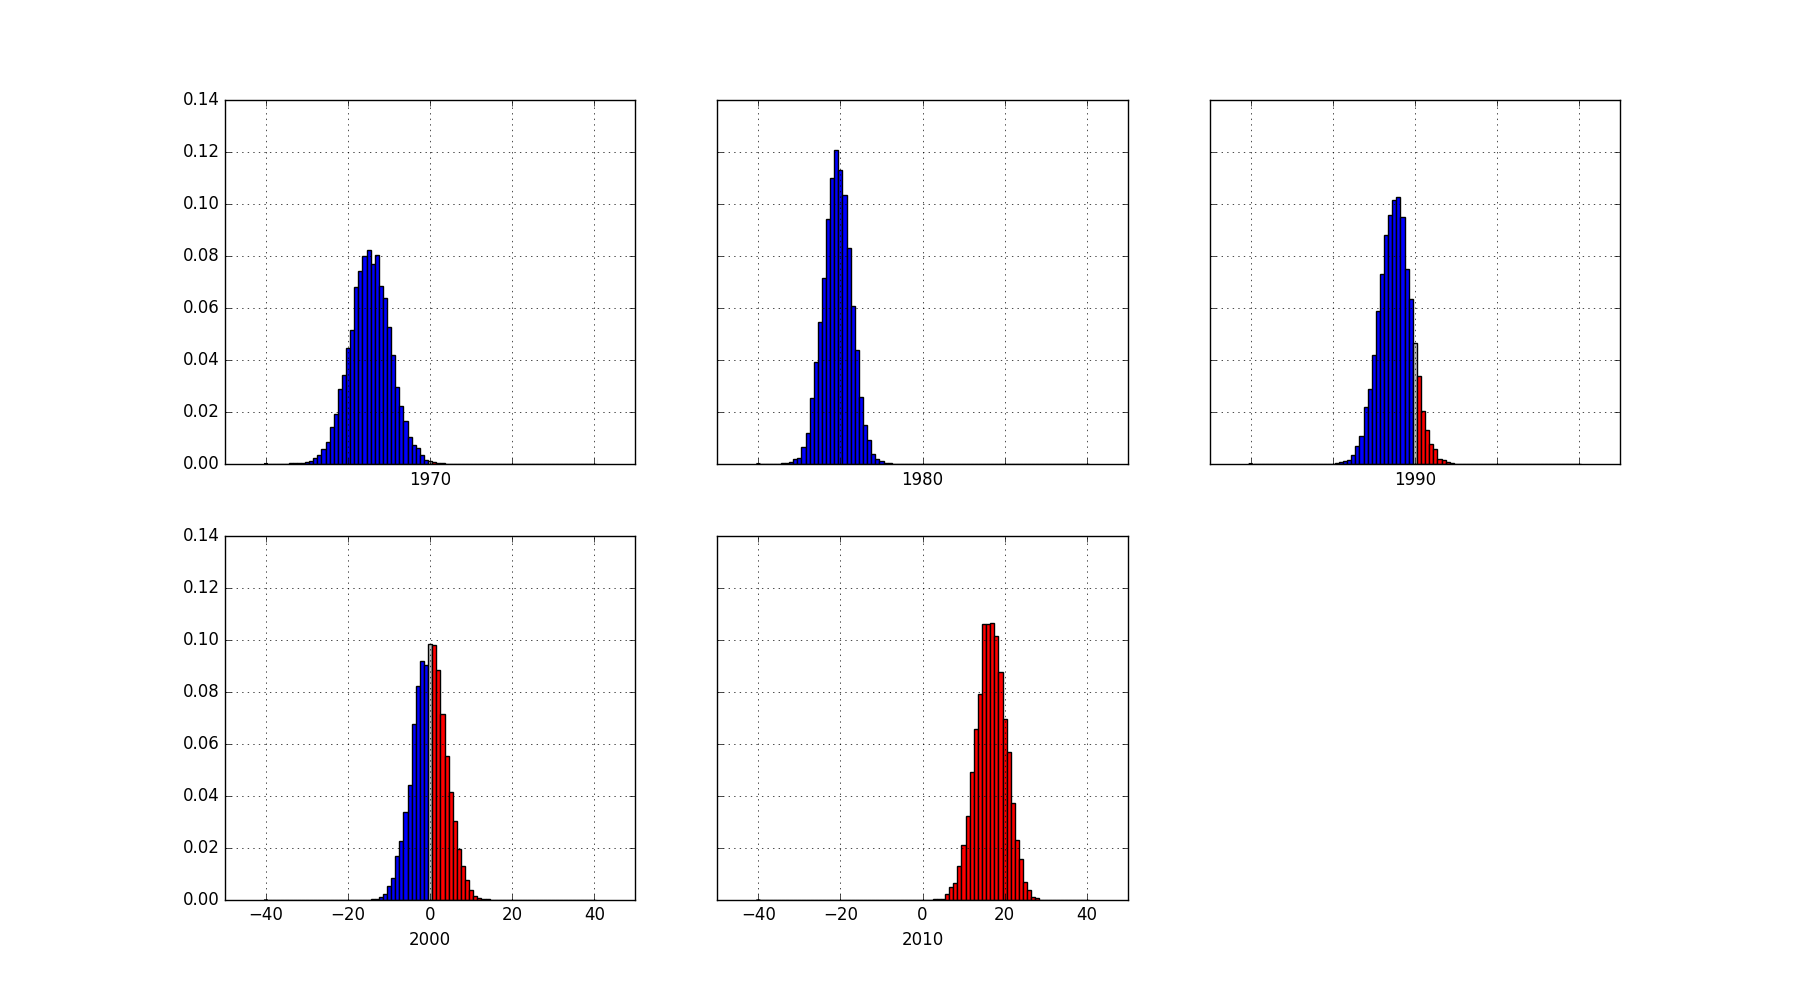
\includegraphics[scale=0.4]{../Figures/ExpectedAsymmetry/netAsymHist.png}
        \caption{Net national asymmetry based on 10,000 simulations}\label{fig:NetAsymHist}
    \end{center}
\end{figure}

\section{Partisan Bias in the Wisconsin State Assembly, post 2010 census\label{sec:Wis}}

\section{Conclusions}

\clearpage
\section*{Acknowledgment}
\section*{}
%\bibliographystyle{plainnat}
%\bibliography{Hyperelas,Bib2}
\clearpage



\end{document}
